\section{Agile Development}\label{sec:agile}

LSST data management follows a long term plan with six month cycles. The  development approach falls in the rather  broad \emph{Agile} methodology. It is also beholden to organizations such as NSF which require a more traditional approach to project development such as the Earned Value Management System (EVMS).
We have presented this from both  the ESA and LSST perspective in SPIE previously  \cite{2014SPIE.9150E..1EG}.
In 2016  we presented a more complete approach for LSST to the problem of Agile in the earned value world \cite{2016SPIE.9911E..0NK}, here we provide just a brief update on that paper concentrating more on the Agile aspects.


\subsection{Management}
The Project Management Guide \cite{DMTN-020} provides  comprehensive details on the mechanisms underpinning LSST Data Management’s approach to project management, the reader is referred to to that document for gory details as required.
Each institution in the DM team is typically
responsible for 1 or more Level 2 WBS elements, and each institution has a Technical/Control Account Manager
(T/CAM) responsible for planning, estimating, monitoring and EVM reporting for that Level 2 WBS element.
The detailed management plan is in LDM-294\cite{LDM-294}.

\subsection{Basic Assumptions}
The Project assumes that a full-time individual works for a total of
1,800 hours per year: this figure is \emph{after} all vacations, sick
leave, etc are taken into account. Staff appointed to ``developer''
positions are expected to devote this effort directly to LSST.

Appointment as a \emph{scientist} includes a 20\% personal research time
allowance. That is, scientists are expected to devote 1,440 hours per
year to LSST, and the remainder of their time to personal research.

Our base assumption is that 30\% of an individual's LSST time (i.e., 540 hours/year for a developer, 432 hours/year for a scientist) are devoted to overhead for regular meetings\footnote{``Meetings'' include, for example, scheduled weekly team meetings, stand-ups, etc.; major conferences or project meetings involving preparation, travel time, etc., should be scheduled in advance and allocated Story Points}, ad-hoc discussions and other interruptions.
This is similar to the standard \emph{Agile} discount, however in the earned value world that must be accounted for and it is considered Level of Effort (LOE)


\subsection{Long Term Planning}
\label{sec:long-term-plan}

The plan for the duration of construction is embodied in:

\begin{enumerate}
\item
  A series of \emph{planning packages}, which describe major pieces of
  technical work. Planning packages are associated with concrete, albeit
  high-level, deliverables (in the shape of milestones), and have
  specific resource loads (staff assignments), start dates, and
  durations. The entire DM system is covered by around 100 of these
  planning packages.
\item
  \emph{Milestones} represent the delivery or availability of specific
  functionality. Each planning package culminates in a milestone, and
  may contain other milestones describing intermediate results.
\end{enumerate}

Planning packages are defined at the fourth level of the Work Breakdown Structure (WBS).

All WBS elements are related to the set of Data Management Products embodied in the System Design \cite{LDM-148} a high level summary of which is given in
Figure \ref{fig:prods}. Each product has a product owner to guide the agile development, this is frequently one of the Data Management Scientists.

\begin{figure}[htbp]
        \begin{center}
                 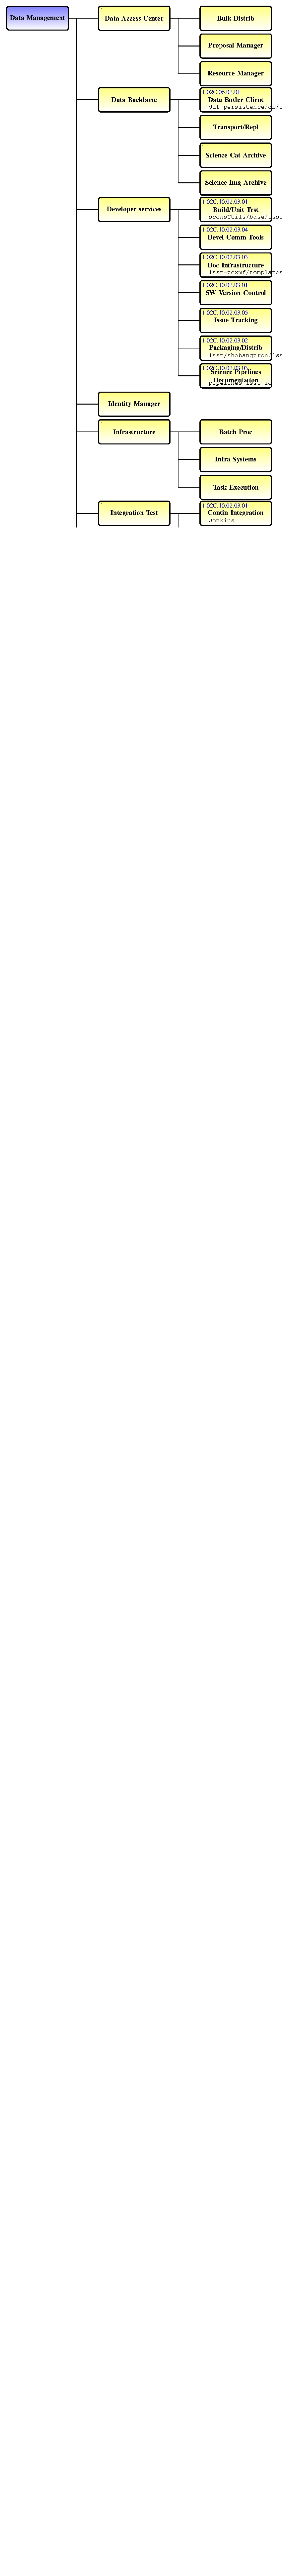
\includegraphics[height=10cm]{ProductTree}
                 \caption{DM product tree. \label{fig:prods} There are over 200 products in the full tree, this diagram shows a truncated form of the product tree to convey an idea of the products.
         }

         \end{center}
 \end{figure}

During the cycle planning process  effort is drawn from the budget embodied in the planning packages to generate the cycle plan, described in terms of epics in Jira.
Each epic itself has a particular budget.
This budget is subtracted from that available in the planning package at the point when the epic is defined.
Team members then add specific stories to these epics.

The Jira system is synchronized with the Primavera project management tool every three months using in-house tools.

In order for the DM system to reach its science goals, new algorithmic or engineering approaches must sometimes be researched.
It is appropriate to budget time for this research work in planning packages and they result in epics of defined length (rather than specific  deliverable).
Areas where successful delivery of the DM system is dependent on speculative research are a source of risk: where possible, the plan  also provides for a fallback option to be taken when research objectives are not achieved.
This may also lead to an entry in the risk register.


Some work is \emph{emergent}: we can predict in advance that it will be necessary, but we cannot
predict exactly what form it will take. The typical example of this is fixing bugs: we can reasonably
assume that bugs will be discovered in the codebase and will need to be addressed,
but we cannot predict in advance what those bugs will be.
We included this in the schedule by defining a \emph{bucket} epic in which stories can be created
when necessary during the course of a cycle.

\subsection{Sprinting} \label{sec:spront} \label{sec:jira_ticket}
The broad plan (to 2022) is laid out in planning packages.
For a  given  cycle (six months)   more detail is put in the form of epics which  are shared across the teams in a face to face meeting a little ahead of the start of cycle.  The team then start to populate the epics with stories (both of which are Jira tickets)  which are at an appropriate level for day to day planning.
Within the cycle we follow monthly sprints with the usual agile steps:
\begin{enumerate}
\item \textbf{Preparation:} Stories for the sprint are chosen and distributed to team members according to available points. This is usually a local team meeting.
\item \textbf{Execution:} As the cycle progresses daily standups are used to catch blockers and clarify stories. At the higher level there are two T/CAM standups each week on Tuesday and Friday to raise issues across team boundaries.
\item \textbf{Review:} At cycle end a retrospective should be conducted.
\end{enumerate}

We use Jira's
\href{https://www.atlassian.com/software/jira/agile}{Agile} capabilities
to manage our sprints. Each technical manager is responsible for
defining and maintaining their own agile board. The board may be
configured for either
\href{https://en.wikipedia.org/wiki/Scrum_(software_development)}{Scrum}
or \href{https://en.wikipedia.org/wiki/Kanban_(development)}{Kanban}
style work as appropriate.

\subsection{Reporting}
DM produces a mandatory written monthly report for NSF/DOE in which each team reports on progress and issues. A new addition to this report since last year is to clearly track the state of milestones which have been met or delayed.
As the previous SPIE paper \cite{2016SPIE.9911E..0NK} pointed out the Primavera system outputs standard project metrics on variance and budget.
Though this is reasonable  for reporting hardware based activities it does not report well on Agile progress unless there are well defined deliverables.
In 2017 we have undertaken to lay out a set of test driven milestones to show progress in Data Management. These milestones are completed by execution of tests laid out in a test specification tying them to requirements, resulting in a test report.
